\documentclass[10pt]{article}      % Use this line for a4 paper

\usepackage{amsmath,amssymb,euscript,yfonts,psfrag,latexsym,dsfont,graphicx}
\usepackage{bbm,color,amstext,wasysym,parskip,balance}
\usepackage{subcaption}
\usepackage{url}
\usepackage[pdftex,hidelinks]{hyperref}
\usepackage{float}

%\usepackage{amsthm}
%\usepackage{refcheck}
%\usepackage{showkeys}
%\usepackage{epstopdf,hyperref,pdfsync,url}
%\graphicspath{{./},{./figures/},{./Matlab/}}




\newtheorem{thm}{Theorem}
\newtheorem{cor}[thm]{Corollary}
\newtheorem{conj}[thm]{Conjecture}
\newtheorem{lemma}[thm]{Lemma}
\newtheorem{prop}{Proposition}
\newtheorem{problem}[thm]{Problem}
\newtheorem{remark}[thm]{Remark}
\newtheorem{defn}[thm]{Definition}
\newtheorem{ex}[thm]{Example}

\newcommand{\mR}{{\mathbb R}}
\newcommand{\mD}{{\mathbb D}}
\newcommand{\cH}{{\mathcal H}}
\newcommand{\E}{{\mathbb E}}  % this is for expectation -- we can change
\newcommand{\bx}{{\mathbf x}}
\newcommand{\mE}{{\mathbb E}}
\newcommand{\cD}{{\mathcal D}}
\newcommand{\cN}{{\mathcal N}}
\newcommand{\cM}{{\mathcal M}}
\newcommand{\cR}{{\mathcal R}}
\newcommand{\cS}{{\mathcal S}}
\newcommand{\cC}{{\mathcal C}}
\newcommand{\cP}{{\mathcal P}}
\newcommand{\cU}{{\mathcal U}}
\newcommand{\cL}{{\mathcal L}}
\newcommand{\cT}{{\mathcal T}}
\newcommand{\diag}{\operatorname{diag}}
\newcommand{\tr}{\operatorname{trace}}
\newcommand{\f}{{\mathfrak f}}
\newcommand{\g}{{\mathfrak g}}
\newcommand{\range}{\cR}
\newcommand{\rH}{{\rm H}}
  %{\operatorname{range}}
\newcommand{\trace}{\operatorname{tr}}
\newcommand{\argmin}{\operatorname{argmin}}

%\newcommand{\ignore}[1]{}

%\def\spacingset#1{\def\baselinestretch{#1}\small\normalsize}
%\setlength{\parskip}{10pt}
%\setlength{\parindent}{20pt}
%\spacingset{1}

%\newcommand{\mike}{\color{magenta}}
%\newcommand{\mmike}{\color{blue}}
%\newcommand{\jk}[1]{{\color{red}{#1}}}

%\newcommand{\rike}[1]{{\color{red}{#1}}}
%\newcommand{\rike}{\color{red}}

\definecolor{grey}{rgb}{0.6,0.6,0.6}
\definecolor{lightgray}{rgb}{0.97,.99,0.99}

%\IEEEoverridecommandlockouts
%\overrideIEEEmargins

%\renewcommand{\baselinestretch}{0.985}

%\def\spacingset#1{\def\baselinestretch{#1}\small\normalsize}
\setlength{\parskip}{5.3pt}
%\setlength{\parindent}{10pt}
%\spacingset{1}

\setlength{\voffset}{2pt}

\title{FLIR project - modeling noise in bolometer signal}
\author{
Project group (alphabetic order): \and
Carl Ringqvist$^1$ \texttt{carrin@kth.se} \and
Giampaolo Mele$^1$ \texttt{gmele@kth.se} \and
H\aa kan Carlsson$^1$ \texttt{hakcar@kth.se} \and
Johan Karlsson$^1$ \texttt{johan.karlsson@math.kth.se} \and
M\"arta Barenthin Syberg$^2$ \texttt{Marta.BarenthinSyberg@flir.se} \and
Olof Runborg$^1$ \texttt{olofr@nada.kth.se} \and
Per Enqvist$^1$ \texttt{penqvist@kth.se} \and
Ulf W\aa llgren$^2$ \texttt{ujgwallgren@gmail.com}
}

\date{%
    $^1$KTH\\%
    $^2$FLIR\\[2ex]%
    \today
  }
% Comment colours
\usepackage{xcolor}
\newcommand{\gm}[1]{{\color{blue}#1\color{black}}}

\begin{document}


\maketitle

\begin{abstract}
A microbolometer is a device for measuring the power of incident
electromagnetic radiation via the heating of a material with a
temperature-dependent electrical resistance in infrared (IR)
cameras. The change in the resistance is measured with an applied bias
voltage, which yields a current that is fed to an integrator. The
integrator then yields a readout voltage that represents the output
signal of the system. The bias voltage also heats the resistance, and
thus in the uncooled microbolometer system, the bias voltage is only applied
periodically to allow the resistance to cool down. In the camera, an
array of bolometers gives an IR image. Based on the heat equation and
the Stefan Boltzmann law of black-body radiation, models can describe
the underlying behavior of the
bolometer, before the readout voltage. We would like to investigate if
the underlying bolometer parameters can be identified using readout
voltage data. Further, we investigate how noise affects the system and
how the models can be modified to account for the noise. A
better understanding of the components and the noise phenomena could potentially
yield better detectors. This report is done in
collaboration with FLIR, based in T\"aby. FLIR develops and produces
cameras for temperature
measurement.

\end{abstract}

%%% Local Variables:
%%% mode: latex
%%% TeX-master: "main"
%%% TeX-PDF-mode: 1
%%% TeX-PDF-via-dvips-ps2pdf: 1
%%% End:

\section{Introduction}


\subsection{The IR camera}
Electromagnetic radiation of wavelengths between $700$ nanometer to
$1$ millimeter comprise what is usually referred to as
\textit{infrared light}. Much like the normal camera is able to detect
and display variations of visible light ($400$ nanometers to $700$
nanometers), infrared cameras produce pictures colored
according to the variations in infrared radiation (IR) of a
scene. Since infrared emission from an object is closely related to
its temperature, an IR camera essentially produces a heat map to the
eye, coloring parts of a scene relative to temperature. For instance
in Figure~\ref{fig:cat}, a cat is depicted based on the IR radiation
it emits. Many infrared
cameras are also able to accurately estimate the temperature of an
object in addition to depicting it.


\begin{figure}[h]
\begin{center}
\includegraphics[height=5cm]{gfx/cat.png}
\caption{Infrared picture of a cat sitting on a table during
  night. The warmblooded cat is clearly distinguished from its cold
  surrounding, making the cat visible to the IR camera although not
  visible to the eye. Source:
  https://www.scienceabc.com/}~\label{fig:cat}
\end{center}
\end{figure}

Infrared cameras are used widely within industrial and military
applications, enabling or enhancing tasks such as dark vision, heat
leakage detection, moisture detection, chemical spill leakage
detection and firefighting. An overview about different devices
together with a catalog can be found in~\cite{flir_handbook}. There
exist mainly two types of techniques for infrared cameras: thermal
detectors and quantum detectors. We will here focus solely on thermal
detectors, and especially the \textit{uncooled bolometer}. A bolometer consists of a plate (pixel)
made of metal or semiconductor material, which for instance could be a mixture of
silicon nitride and vanadium oxide. This plate is suspended in the air
via two supporting legs that is connected to a substrate. The
supporting legs are also connected to a voltage
source. The structure is depicted in Figure~\ref{fig:structure}. Incoming infrared radiation is focused via a lens to the
plate, causing it to be heated, which in turn alters its
resistance. This change in resistance can be measured through an
input voltage and the resulting current is a function of the strength
of the incoming infrared radiation and hence
the temperature of the emitting scene.

\begin{figure}[h]
\begin{center}
\includegraphics[height=5cm]{gfx/pixel1.png}
\caption{Physical structure of the bolometer~\cite{xiu2010research}.}~\label{fig:structure}
\end{center}
\end{figure}

\subsection{Project description}

The project aims to establish a mathematical relationship between the
temperature of an object and the resulting bolometer signal. Briefly,
the incoming radiation of an object, described by the Stefan-Boltzmann
law, heats up the bolometer, which can be described by the heat
equation. The applied voltage is used to measure the change in
resistance due to the temperature change. More precisely, the
output signal is a voltage from an integrator, that can be used to
retrieve the change in the resistance and thus via the heat equation
and the Stefan-Boltzmann law the temperature of the target. An explicit
description of the output signal is given in
Section~\ref{sec:model_disc}.

In reality however, the output signal is noisy. The project aims to
incorporate noise into the model in a manner consistent with data and
experience. A good model of the noisy signal might for example enable
applying an efficient filtering algorithm that reduces noise. The project's aim is to investigate how a noisy input signal affects the output signal.

More precisely in this project we:
\begin{itemize}
 \item simulate the read-out signal of the bolometer by solving the differential equations modeling the problem,
 \item reproduce numerical simulations that fits with empirical experiments,
 \item model and analyze the noise in the differential equations,
 \item reproduce numerical simulations (with noise) that fits with empirical experiments.
\end{itemize}

%%% Local Variables:
%%% mode: latex
%%% TeX-master: "main"
%%% TeX-PDF-mode: 1
%%% TeX-PDF-via-dvips-ps2pdf: 1
%%% End:
			% Carl
\setlength{\belowcaptionskip}{-15pt}
\setlength{\abovecaptionskip}{0pt}
\section{Model and discretization} \label{sec:model_disc}

Each pixel of an IR camera can be modeled as the circuit in Figure~\ref{fig:circuit}.
\begin{figure}[ht]
 \includegraphics[scale=0.31]{gfx/circuit.png}
\caption{Circuit schematic that model a pixel of the IR camera generated with \url{https://www.digikey.com/schemeit}.}
\label{fig:circuit}
\end{figure}
More precisely the bolometer corresponds to the resistor R2. 

The pixel of the IR camera works as follow: a bias voltage is applied as square signal. The voltage is a piecewise constant function defined as 
\begin{align} \label{eq:Vb}
 V_b(t)&=\begin{cases} v_b & n t_f < t < n t_f + t_i \\
 0 &\mbox{ otherwise.} 
 \end{cases} && n \in {\mathbb N}
\end{align}
The readout signal is the voltage $V_{samp}$ across the capacitor C2 that we can express, by using the Kirchhoff's law, as
\begin{align} \label{eq:Vsamp_def}
 V_{samp} = 
 \frac{1}{\tilde C} \int_{n t_f}^{n t_f + t_i} \left( \frac{V_0}{R_S} - \frac{V_b(s)}{R(T(s))} \right) ds + E
\end{align}
where $R(T)$ is the value of the resistance of R2 as function of the temperature and $\tilde C$ is the capacitance of C2. In \cite{xiu2010research} this is modeled as $R(T)=R_S e^{\alpha(T-T_s)}$ where $\alpha$ is a constant that depends on the material of the bolometer. Clearly, in order to compute this integral, we need to know the temperature as function of the time. This relation is described  by the  \emph{heat balance equation} \eqref{eq:heat_balance_equation}.

The output signal can therefore be simulated in the following way. We set an initial temperature $T_0$ for the bolometer and solve the heat balance equation~\eqref{eq:heat_balance_equation}. Then we compute the integral describing the readout signal~\eqref{eq:Vsamp_def}.


\subsection{Illustrative example} \label{sec:example}
A reasonable and realistic simulation of the bolometer response can be obtained by solving the equations~\eqref{eq:heat_balance_equation}-\eqref{eq:Vsamp_def} with the parameters and coefficients given in Table~\ref{tab:par_coeffs_example}. Moreover we have set $T_0=T_s$, $P_t=A_s \sigma (T_0+10)^4$ and $P_s=A_s \sigma T_s^4$.


The solution of~\eqref{eq:heat_balance_equation} is illustrated in Figure~\ref{fig:solution_heat_balance_eq}. In the phase when the bias voltage is active, usually referred as \emph{integration time}, the temperature of the bolometer rises of circa $3K$. This is due to the fact that the current flowing through a component causes its overheat. When the bias voltage is not active, the temperature of the bolometer drops of circa $3K$, therefore we refer to this phase as \emph{cooling time}. See Figure~\ref{fig:solution_heat_balance_eq_splitted} for the illustration this such phenomena. The readout is illustrated in Figure~\ref{fig:Vout}. 

\begin{figure} 
 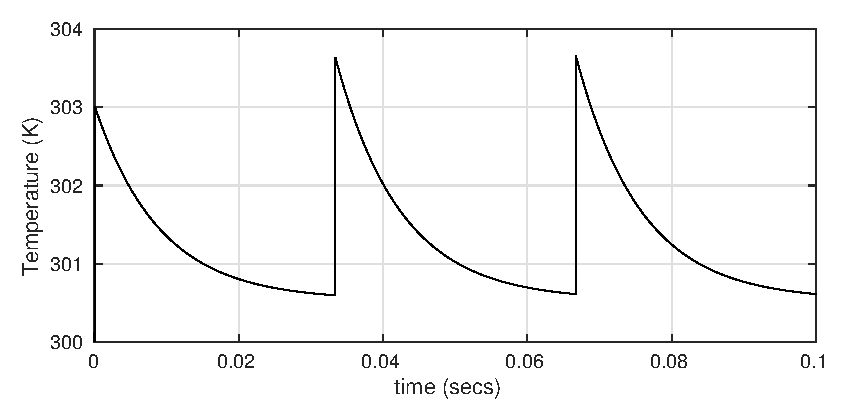
\includegraphics[scale=0.9]{gfx/fig1_several_pulses.eps} 
 \caption{Solution to the heat balance equation~\eqref{eq:heat_balance_equation}.}
 \label{fig:solution_heat_balance_eq}
\end{figure}
\begin{figure} 
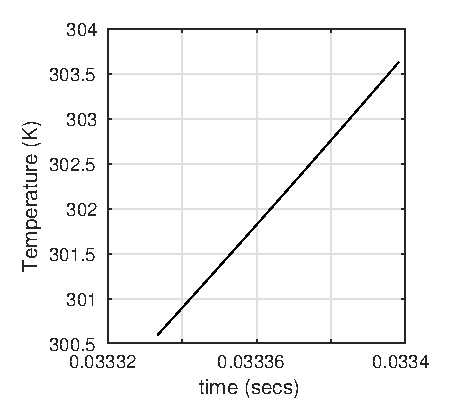
\includegraphics[scale=0.9]{gfx/fig1_int_time.eps} 
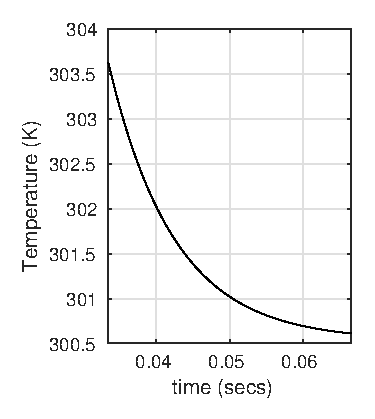
\includegraphics[scale=0.9]{gfx/fig1_cooling.eps}
\caption{Solution to the heat balance equation~\eqref{eq:heat_balance_equation} during the integration time $V_b>0$, and during the cooling time $V_b=0$. }
\label{fig:solution_heat_balance_eq_splitted}
\end{figure}
\begin{figure}
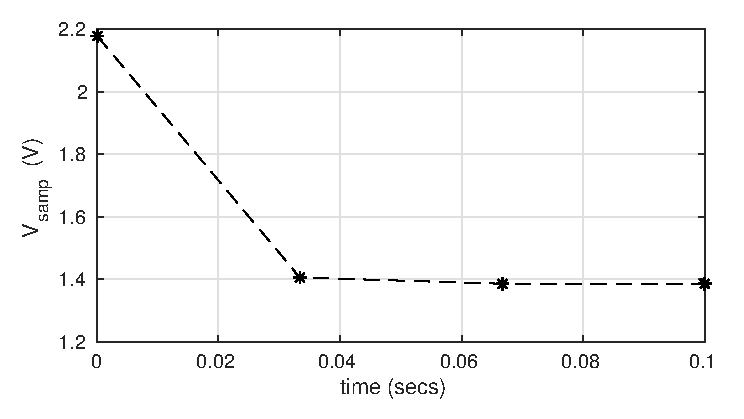
\includegraphics[scale=0.9]{gfx/fig1_Vout_several_pulses.eps} 
\caption{Readout voltage~\eqref{eq:Vsamp_def}.}
\label{fig:Vout}
\end{figure}

As we can see in Figure~\ref{fig:solution_heat_balance_eq}-\ref{fig:solution_heat_balance_eq_splitted}, the temperature of the bolometer does not only depend on the incoming IR radiation, namely the temperature of the object we are observing, but also on the bias voltage. In order to mitigate this phenomena, the frame-time $t_f$ is set much larger than the integration time $t_i$ to avoid overheat the bolometer. In particular the function temperature $T$ oscillates in the time (after very few pulses) around the temperature due to the incoming IR radiation. This also reflects in the readout, since $V_{samp}$ becomes constant, i.e., the bolometer has cached the temperature of the observed object.

\begin{center}
\begin{table}[]
\centering
\caption{Parameters and coefficients used in Section~\ref{sec:example}}
\label{tab:par_coeffs_example}
\begin{tabular}{|c|cr|c|cr|}
\hline
 $t_i$ 		& $65$ 		& $  \mu sec$ 		& $\alpha$  	&    	$-0.02$	&			\\
\hline 
 $tf$ 		& $1/30$ 	& $  sec$ 	 	& $e$ 		&    	$0.8$ 	&			\\
\hline 
 $R_S$ 		& $800 $ 	& $  k \Omega$ 		& $A$ 		&    	$17  $ 	& $ \mu m$ (square)	\\
\hline 
 $T_s$		& $300 $ 	& $  K$ 	 	& $A_s$ 	&    	$17  $ 	& $ \mu m$ (square)	\\  
\hline 
 $G_{leg}$	&  $250 $ 	& $   \mu W K^{-1}$	& $\tilde C$ 	&	$4$ 	& $   p F$		\\   
\hline 
 $C$		&  $25 $ 	& $   n J K^{-1}$ 	& $V_0$		& 	$3.1$ 	& $   V$		\\
\hline 
 $v_b$		& $3 $ 		& $   V$		& $E$		& 	$2$ 	& $   V$		\\
\hline 
\end{tabular}
\end{table} 
\end{center}

\subsection{Numerical methods for simulating the bolometer}
The output signal can be simulated by setting an initial temperature for the bolometer and by solving the heat balance equation~\eqref{eq:heat_balance_equation}. The readout $V_{samp}$ corresponds to the integral~\eqref{eq:Vsamp_def} that can be approximated with any numerical integration algorithm such as Riemann sum, trapezoidal rule, etc. The equation~\eqref{eq:heat_balance_equation} cannot be solved naively with a numerical scheme for ODE described, e.g., in \cite{mattheij1996ordinary,ascher1998computer}. Namely, any \texttt{matlab} ODE solver is not capable of solving~\eqref{eq:heat_balance_equation}. This is due to the fact that the function $V_b(t)$ (bias voltage), defined in~\eqref{eq:Vb}, has a very fast variation. The strategy for effectively solve the problem consists in splitting the domain in sub-domains where $V_b(t)$ is constant. 

Assume that we want to solve~\eqref{eq:heat_balance_equation} for $0 \le t \le m t$ for a fixed $m \in \mathbb{N}$, namely we want $m$ pulses. The time domain can be split as
\begin{align*}
 [0, m t_f] = \bigcup_{k=0}^{m-1} (I_k \cup J_k)
\end{align*} 
where $I_k=[k t, k t_f+t_i]$ and $J_k = [k t_f + t_i, (k+1)t_f]$. 
We set $T_0(0):=T_0$ and for $k=1, 2, \dots$, we solve the ODE in $I_k$
\begin{align} \label{eq:heat_balance_equation_seq_bias}
& C\frac{dT_{k+1}}{dt}=\frac{v_b^2}{R(T_{k+1})}+\epsilon_e(P_t+P_s -2A\sigma T_{k+1}^4)-G_{leg}(T_{k+1}-T_s) \ , \ t \in I_k \nonumber \\
& T_{k+1}(kt_f)=T_{k}(kt_f)&
\end{align}
we set $\alpha:=T_{k+1}(kt_f+t_i)$ and we solve the ODE in $J_k$
\begin{align} \label{eq:heat_balance_equation_seq_no_bias}
& C\frac{dT_{k+1}}{dt}=\epsilon_e(P_t+P_s -2A\sigma T_{k+1}^4)-G_{leg}(T_{k+1}-T_s) \ , \ t \in J_k \nonumber \\
&T_{k+1}(kt_f+t_i)=\alpha_{k+1}	
\end{align}
The solution $T(t)$ of~\eqref{eq:heat_balance_equation} is obtained by gluing the functions $T_j(t)$, i.e., 
\begin{align*}
 T(t) = 
 \begin{cases}
  T_0(t) & t \in I_0 \cup J_0	\\
  T_1(t) & t \in I_1 \cup J_1	\\
	 & \vdots 		\\
  T_1(t) & t \in I_k \cup J_k	\\
	 & \vdots		\\
  T_m(t) & t \in I_m \cup J_m	\\
 \end{cases}
\end{align*}
In conclusion, the solutions of the ODEs~\eqref{eq:heat_balance_equation_seq_bias}-\eqref{eq:heat_balance_equation_seq_no_bias} can be approximated with any numerical scheme such us Euler method, Runge--Kutta, etc. We did not observe any difficulty in solving these equations and we chose the explicit Euler method as solver since this can easily be extended to the noised model (stochastic differential equation) that we will introduce in the next section.  

		% Giampaolo
\section{Model with noise and discretization}

There are several sources of noise in a micro-bolometer setup:
\begin{itemize}
\item Thermal noise in the resistances,
\item Flicker noise in resistances,
\item Burst noise,
\item Thermal fluctuations in the bolometer temperature,
\item Noise in incident IR radiation,
\item Noise in read out circuits.
\end{itemize}

In this report we shall only consider the first two types of noises,
thermal and flicker noise in resistances.

\subsection{Thermal noise}

Any resistance with a temperature $T$ above zero, will cause the
charge carriers in the material to fluctuate. The fluctuations are
independent of each other, and will generate a current with a
voltage. This phenomenon is referred to as thermal noise, but is also
known as white noise and Johnson noise. This type of noise was first
discovered by the Swedish engineer John
B. Johnson~\cite{PhysRev.32.97}, and his colleague Harry Nyquist, also
swedish, provided a theory for the noise based on statistical
physics\cite{PhysRev.32.110}. One of the characteristics of the noise,
is the flat power spectrum for all most all frequencies, which is also
characteristic for white light.

In electrical circuits, thermal noise is commonly modeled as an additional
power source in series with the resistance, see Figure~\ref{fig:johnsonEquivalentNoise}.
\begin{figure}
  \centering
  \includegraphics[width=0.5\textwidth]{gfx/JohnsonNoiseEquivalentCircuits.png}
  \caption{Equivalent model for thermal noise in a resistor.}~\label{fig:johnsonEquivalentNoise}
\end{figure}
Due to the random nature of the additional power source, it is not
possible to predict the instantaneous voltage produced, but instead the
average behavior. Nyquist\cite{PhysRev.32.110} found that the power
spectrum of thermal noise to be
\begin{equation}
  \label{eq:power_spectrum_white_noise}
  S(f) = 4 k_B T R,
\end{equation}
where $k_B$ is the Boltzmann constant, $T$ is the temperature of the
resistance, and $R$ is the resistance. The total contribution of the
noise source is then calculated by summing up the contribution from
each frequency component.
\begin{equation}
  \label{eq:2}
  \E \left[ V^2 \right] = \int_B S(f) \mathrm(d) f,
\end{equation}
where $B$ is the bandwidth of the circuit.

% The mean square square voltage o

A statistical model commonly used to white noise is a stationary stochastic
process where the auto-correlation function is
\begin{equation}
  \label{eq:autocorrelation_white_noise}
  R(s,t)={\frac {\operatorname {E} [(X_{t}-\mu _{t})(X_{s}-\mu
      _{s})]}{\sigma _{t}\sigma _{s}}} =
  \begin{cases}
    \sigma_{t}^2 , \quad t = s, \\
    0 , \quad t \neq s
  \end{cases}
\end{equation}
meaning that the process is uncorrelated in time. A distribution that
can be used for this process is the Gaussian distribution
$\mathcal{N}(0, \sigma)$.

\subsection{Flicker Noise}\label{sec:flicker-noise}

Another type of noise source that exists in circuits is flicker
noise, or also known as low frequency noise, 1/$f$ noise or pink noise. The power
spectrum of the Flicker noise is
\begin{equation}
  \label{eq:power_spectrum_flicker_noise}
  S(f) \propto \frac{k}{f^{\alpha}}.
\end{equation}
where $\alpha \in [0.5, 1.5]$ and $k$ is a material constant.

One explanation of the occurrence of the flicker noise in resistors is
that the charge carriers get trapped in capture sites of the
conductor, and are then released with variable rates. This was first
explained by Schottky for flicker noise in vacuum tubes~\cite{PhysRev.28.74}.

To generate the flicker noise in simulation there are several methods
available, listed in~\cite{381848}.

\subsection{Noise model and simulation scheme}

To compensate for the noise in the read-out circuit, one first has to
determine how noise enters the differential equation governing the
behavior of the system. The simplest possible solution is of course to
add a noise term of a normally distributed character to the left hand side
in Equation~\eqref{eq:heat_balance_equation}, rendering the theory for
diffusion processes readily available. More precisely we rewrite Equation~\eqref{eq:heat_balance_equation}
as
\begin{align} \label{eq:heat_balance_equation_noise1}
 CdT&=\left(\frac{V_b(t)^2}{R(T)}+\varepsilon(P_t+P_s -2A_s \sigma
      T^4)-G_{leg}(T-T_s)
      \right)dt + K(t)dW \\
 T(0)&=T_s	\nonumber
\end{align}
where $K$ is a function of time, and $W \sim N(0, dt)$.
The function $K(t)$ is chosen according to the following heuristic.
We expect the noise in the output to be the cause of resistor fluctuations.
Motivated by the setup for Figure~\ref{fig:johnsonEquivalentNoise}, we thus redefine the voltage over
the bolometer resistance as
\begin{equation}
  \label{eq:randomvariable_transformation}
  V \rightarrow V_0 + \Delta V,
\end{equation}
where $V_0$ is the noise-less resistance over the voltage, and $\Delta
V$ is a random variable representing the random fluctuations in the
voltage.

We thus want noise to enter the heat equation in Equation~\eqref{eq:heat_balance_equation}
roughly as
\begin{equation}
  \label{eq:heat_balance_equation_noise}
  C\frac{dT}{dt}=\frac{(V_b(t) + \Delta V)^2}{R(T)}+ f(T),
\end{equation}
where $\Delta V$ is the added noise term, accounting for the
fluctuations in the resistance $R(T)$ and $f(T)$ are the other terms
in Equation~\eqref{eq:heat_balance_equation}.
Expanding the square we get the equation
\begin{equation}
  \label{eq:heat_balance_equation_noise_SDE1}
  C\frac{dT}{dt}=\frac{1}{R(T)} (V_b^2(t) + 2 V_b(t) \Delta V + (\Delta V)^2) + f(T),
\end{equation}
If the squared noise term is negligible in the limit, we are left with
\begin{equation}
  \label{eq:heat_balance_equation_noise_SDE2}
  C\frac{dT}{dt}=\frac{1}{R(T)} (V_b^2(t) + 2 V_b(t) \Delta V  ) + f(T)
\end{equation}
Thus we chose $K(t)$ in Equation~\eqref{eq:heat_balance_equation_noise1}
as $K(t) = 2 V_b(t) \sigma$, where $\sigma$ is a parameter to be calibrated or
physically motivated. The noisy heat development can now be simulated
in a well defined setting, with the dynamics independent of step size $\Delta t$:

\begin{align} \label{eq:heat_balance_equation_noise_discr}
 CT_{i+1}&=\left(\frac{V_b(t_{i})^2}{R(T_{i})}+\varepsilon(P_t+P_s -2A_s \sigma T^4)-G_{leg}(T-T_s)\right)\Delta t + 2 V_b(t) \sigma \sqrt{\Delta t} W \\
 T(0)&=T_s	\nonumber
\end{align}

where $W \sim N(0,1)$.


%%% Local Variables:
%%% mode: latex
%%% TeX-master: "main"
%%% TeX-PDF-mode: 1
%%% TeX-PDF-via-dvips-ps2pdf: 1
%%% End:
 	% Håkan Carlsson
\section{Numerical experiments}
\subsection{Solution with noisy model}
Plots from running the temperature simulation and succeeding integrator with the noisy scheme outlined in Equation~\eqref{eq:heat_balance_equation_noise_discr} are shown
in Figure~\ref{fig:noisysol}. We see that the difference from the deterministic solution is marginal. 
\begin{figure}
 \begin{center}
%\begin{minipage}[t]{0.35\textwidth}
\includegraphics[scale=0.35]{gfx/int_time.jpg} 
%\hfill
%\end{minipage}
%\begin{minipage}[t]{0.35\textwidth}
\includegraphics[scale=0.35]{gfx/cooling.jpg}
%\end{minipage}
%\\
\includegraphics[scale=0.35]{gfx/several_pulses.jpg}
\includegraphics[scale=0.35]{gfx/vsamp.jpg}  	
  \caption{Temperature and output signal development over time. Red: Noisy solution, Black: Deterministic solution}
  \label{fig:noisysol}
  \end{center}
\end{figure}

%\begin{center}
%\begin{minipage}[t]{0.35\textwidth}
%\includegraphics[scale=0.35]{gfx/int_time.jpg} 
%\hfill
%\end{minipage}
%\begin{minipage}[t]{0.35\textwidth}
%\includegraphics[scale=0.35]{gfx/cooling.jpg}
%\end{minipage}
%\\
%\includegraphics[scale=0.35]{gfx/several_pulses.jpg} 	
%\end{center}

\begin{center}
\includegraphics[scale=0.35]{gfx/vsamp.jpg} 	 
\end{center}

\begin{center}
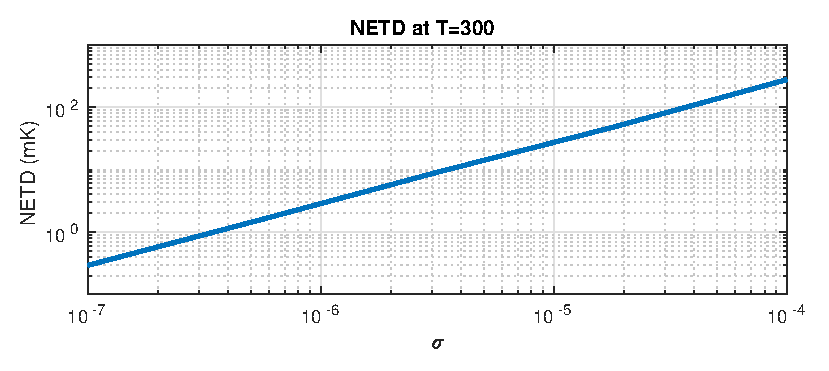
\includegraphics[scale=0.35]{gfx/NETD_as_function_of_sigma.eps} 	 
\end{center}

\begin{center}
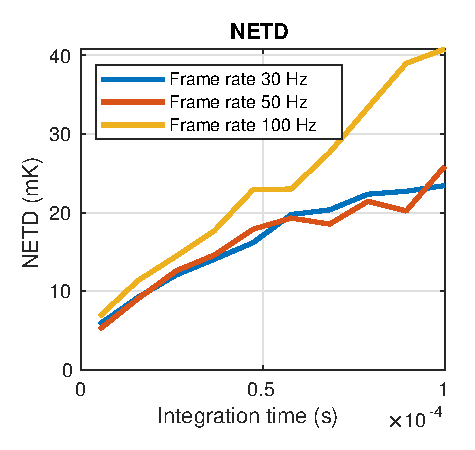
\includegraphics[scale=0.35]{gfx/NETS_Function_of_Integration_Time.eps} 	 
\end{center}

\begin{center}
\includegraphics[scale=0.35]{gfx/Response_Function_of_Integration_Time.eps} 	 
\end{center}

\begin{center}
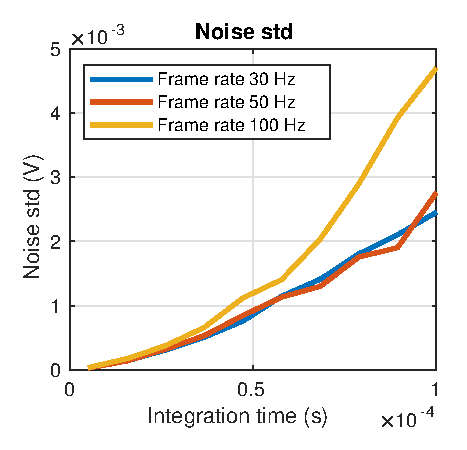
\includegraphics[scale=0.35]{gfx/STD_Function_of_Integration_Time.eps} 	 
\end{center}

\begin{center}
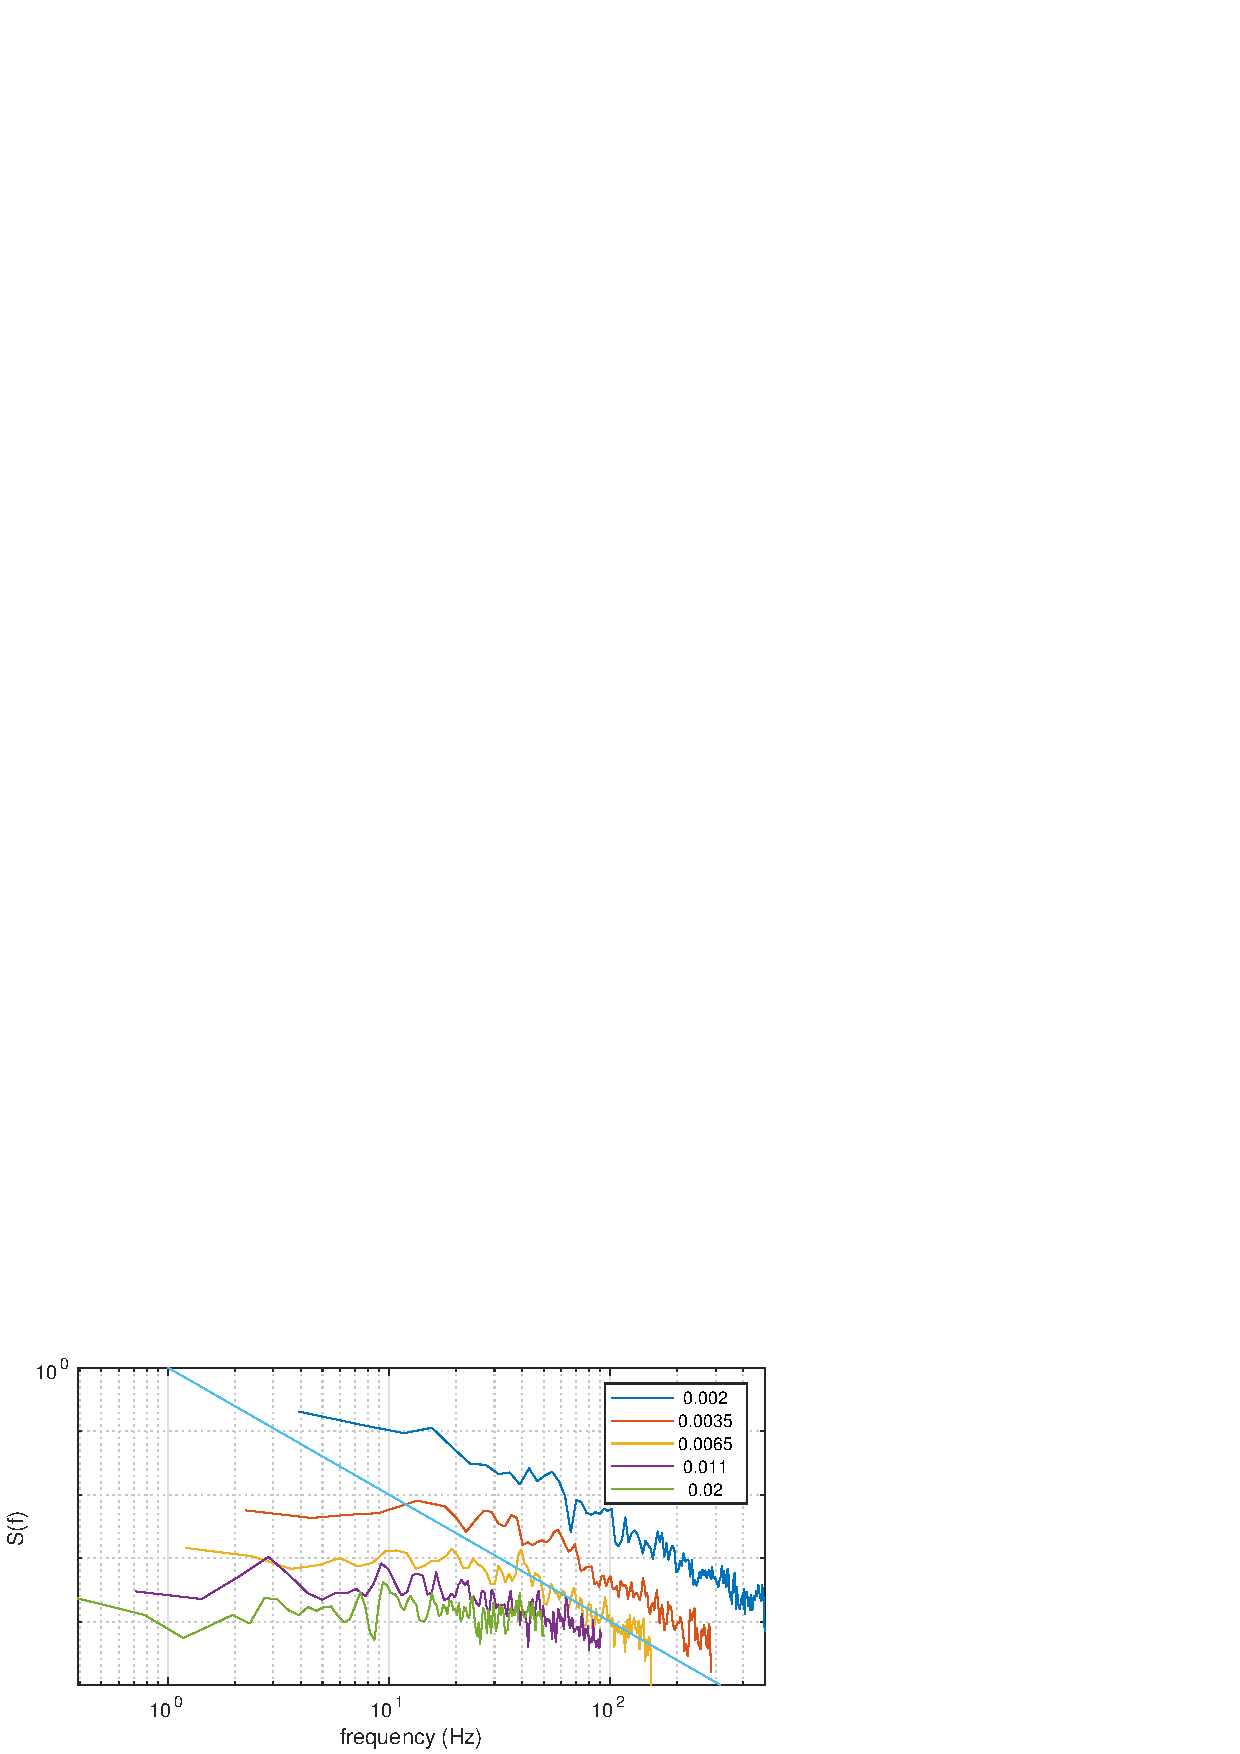
\includegraphics[scale=0.35]{gfx/pspec.png} 	 
\end{center}

\begin{center}
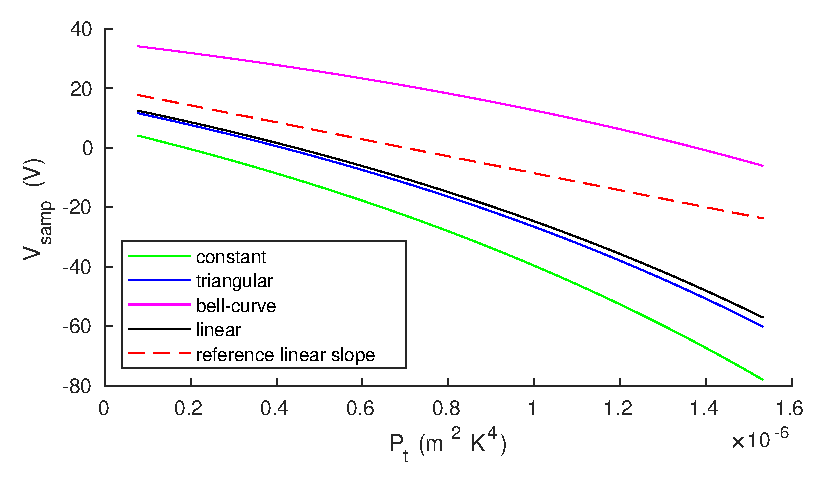
\includegraphics[scale=0.2]{gfx/out_vs_inrad} 	 
\end{center}

%\begin{figure}[h]
%\begin{center}
%\includegraphics[height=5cm]{gfx/int_time.jpg}
%\caption{}
%\end{center}
%\end{figure}
%
%\begin{figure}[h]
%\begin{center}
%\includegraphics[height=5cm]{gfx/cooling.jpg}
%\caption{}
%\end{center}
%\end{figure}
%
%\begin{figure}[h]
%\begin{center}
%\includegraphics[height=5cm]{gfx/several_pulses.jpg}
%\caption{}
%\end{center}
%\end{figure}		% Carl
\section{Outlook and future extensions}

\subsection{Noise process inclusion}
In section 3 we went through the heuristic underlying the inclusion of
noise in the model. This heuristic is however not entirely
satisfactory. Although one can certainly argue for the negligibility
of the squared noise term, it was dropped rather ad hoc. Neither did
we account for the fact that the noise as inserted in the heuristics
is subject to multiplication by a $dt$-term in the actual simulation,
making it hard to establish a scaling scheme for the noise term with a
well defined stochastic limit as step-size goes to 0. What we need in
order to fully solve this matter is stochastic calculus.


Consider thermal noise and assume that the bias voltage $V(t)$ can be
described as a diffusion process. Thermal noise has a white noise
behavior, so ideally, stochasticity around the mean of the bias
voltage $V_{m}(t)$ should have white noise form. Unfortunately, white
noise is not possible to write as a diffusion process. We therefore
suggest that $V(t)$ is modelled as follows:


\begin{align*}
d V = k(V_{m}(t)-V(t)) + \sigma dW_{t}
\end{align*}

This is a Ornstein-Uhlenbeck process, which imposes a mean reverting
mechanism. If the process is above $V_m(t)$, the drift term is
negative and the process will tend to move towards $V_m(t)$. If the
process is below $V_m(t)$, the reverse holds true. This makes
correlation variance increase over time limited when comparing to the
standard Brownian e.g. By adjusting the constants $\sigma$ and $k$, we
can generate an erratic process dynamics with mean-adjusted noise much
resembling white noise.


Let us consider what happens with the temperature dynamics in
equation~\eqref{eq:heat_balance_equation} when we assume the function
$V(t)$ has the stochastic dynamics as described above. We are going to
use the Lemma of Ito, which states that if a diffusion process $X$ has
dynamics $dX = \mu(t)dt + \sigma(t)dW_{t}$, then $f(X)$ (under certain
regularity conditions) has dynamics


\begin{align*}
d f = \left(\frac{\partial f}{ \partial t} + \mu(t)\frac{\partial f}{ \partial x} + \frac{\sigma(t)^{2}}{2}\frac{\partial^{2} f}{ \partial^{2} x}\right)dt + \sigma(t)\frac{\partial f}{ \partial x}dW_{t}
\end{align*}

In our case $f(x) = x^{2}$, so $\frac{\partial f}{ \partial t} = 0$, $\frac{\partial f}{ \partial x} = 2x$, $\frac{\partial^{2} f}{ \partial^{2} x} = 2$. Moreover, $\mu(t) = K(V_{m}(t)-V(t))$, and $\sigma(t)=\sigma$.
Plugging in these values in the Ito formula gives

\begin{align*}
d f = ( k(V_{m}(t)-V(t))2V(t) + \sigma^{2})dt + \sigma(t)2V(t)dW_{t}
\end{align*}

or

\begin{align*}
d X(t)= ( k(V_{m}(t)-\sqrt{X(t)})2\sqrt{X(t)} + \sigma^{2})dt + \sigma(t)2\sqrt{X(t)}dW_{t}
\end{align*}

Note that the temperature dynamics constitute a well defined
stochastic process with the deterministic $V$  replaced by the
stochastic function $X$. The replacement operation turns the
deterministic ODE into a diffusion process with another diffusion
process ($X$) as drift coefficient. As $X$ is adapted to the same
underlying filter as $T$, the process is well defined via the Ito
integral.


%%% Local Variables:
%%% mode: latex
%%% TeX-master: "main"
%%% TeX-PDF-mode: 1
%%% TeX-PDF-via-dvips-ps2pdf: 1
%%% End:
				% Carl
\section{Conclusion}

A mathematical model for the temperature evolution of a microbolometer
and the corresponding output voltage was derived. The model is built
using the heat equation, the Stefan Boltzmann's law, and the Joule
heating law. The change in the temperature of the bolometer
is measured through the resistance change. The heat equation model was
modified based on heuristic arguments to include an additive noise
term in the bias voltage, and the resulting differential equation was
discretized and solved using the explicit Euler scheme.

This, however, led to counter intuitive results regarding the NETD and
the power spectrum of the output voltage, raising the question
whenever the assumed stochastic model was accurate
enough. Unfortunately, there was no experimental data available to
verify the numerical simulations to.

Nevertheless, hindsight provided us with a more well defined
stochastic model to model the phenomena. Unfortunately, time was not
enough to try out this idea.


%%% Local Variables:
%%% mode: latex
%%% TeX-master: "main"
%%% TeX-PDF-mode: 1
%%% TeX-PDF-via-dvips-ps2pdf: 1
%%% End:


\bibliographystyle{plain}
\bibliography{main_bib.bib}

\end{document}

%%% Local Variables:
%%% mode: latex
%%% TeX-master: t
%%% TeX-PDF-mode: 1
%%% TeX-PDF-via-dvips-ps2pdf: 1
%%% End:
